% Q11：按固定候选 PDF 第 1 页可见关系重绘。空间位置为示意，不表示比例。
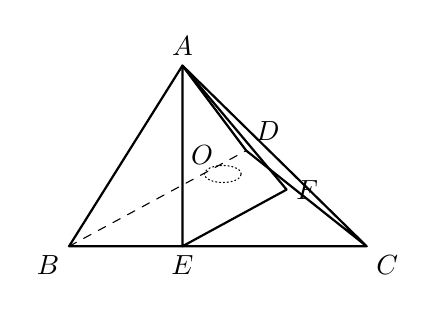
\begin{tikzpicture}[line cap=round,line join=round,scale=0.9]
  \coordinate (A) at (-0.55,2.55);
  \coordinate (B) at (-2.15,0);
  \coordinate (C) at (2.05,0);
  \coordinate (D) at (0.35,1.35);
  \coordinate (E) at (-0.55,0);
  \coordinate (F) at (0.92,0.80);
  \coordinate (O) at (0.02,1.02);

  % 四面体棱与截面；隐藏的棱以虚线表示。
  \draw[thick] (A)--(B) (B)--(C) (C)--(A) (A)--(D) (D)--(C);
  \draw[dashed] (B)--(D);
  \draw[thick] (A)--(E) (E)--(F) (F)--(A);
  % 截面内切球的圆截面，仅表示球心与相切关系，不表示比例。
  \draw[densely dotted] (O) ellipse (0.26 and 0.12);

  \node[above] at (A) {$A$};
  \node[below left] at (B) {$B$};
  \node[below right] at (C) {$C$};
  \node[above right] at (D) {$D$};
  \node[below] at (E) {$E$};
  \node[right] at (F) {$F$};
  \node[above left] at (O) {$O$};
\end{tikzpicture}
